%%%%%%%%%%%%%%%%%%%%%%%%%%% asme2e.tex %%%%%%%%%%%%%%%%%%%%%%%%%%%%%%%
% Template for producing ASME-format articles using LaTeX            %
% Written by   Harry H. Cheng                                        %
%              Integration Engineering Laboratory                    %
%              Department of Mechanical and Aeronautical Engineering %
%              University of California                              %
%              Davis, CA 95616                                       %
%              Tel: (530) 752-5020 (office)                          %
%                   (530) 752-1028 (lab)                             %
%              Fax: (530) 752-4158                                   %
%              Email: hhcheng@ucdavis.edu                            %
%              WWW:   http://iel.ucdavis.edu/people/cheng.html       %
%              May 7, 1994                                           %
% Modified: February 16, 2001 by Harry H. Cheng                      %
% Modified: January  01, 2003 by Geoffrey R. Shiflett                %
% Use at your own risk, send complaints to /dev/null                 %
%%%%%%%%%%%%%%%%%%%%%%%%%%%%%%%%%%%%%%%%%%%%%%%%%%%%%%%%%%%%%%%%%%%%%%

%%% use twocolumn and 10pt options with the asme2e format
\documentclass[twocolumn,10pt]{asme2e}
\usepackage[utf8]{inputenc}
\usepackage{graphicx}
\usepackage{amsmath}
\usepackage{amsfonts}
\usepackage{amsbsy}
\usepackage{todo}
\usepackage{tabularx}
\usepackage{tikz}
\usepackage{nameref}
\usepackage[europeanresistors,americaninductors]{circuitikz}
\renewcommand{\todo}{\Todo}
\newcommand{\vect}[1]{\boldsymbol{#1}}
\newcommand{\tr}{^\intercal}
\special{papersize=8.5in,11in}
\usepackage{url}
\usepackage{epstopdf}

%% The class has several options
%  onecolumn/twocolumn - format for one or two columns per page
%  10pt/11pt/12pt - use 10, 11, or 12 point font
%  oneside/twoside - format for oneside/twosided printing
%  final/draft - format for final/draft copy
%  cleanfoot - take out copyright info in footer leave page number
%  cleanhead - take out the conference banner on the title page
%  titlepage/notitlepage - put in titlepage or leave out titlepage
%  
%% The default is oneside, onecolumn, 10pt, final

%%% Replace here with information related to your conference
\confshortname{OMAE 2015}
\conffullname{the ASME 34th International Conference on Ocean, Offshore and Engineering}

%%%%% for date in a single month, use
%\confdate{24-28}
%\confmonth{September}
%%%%% for date across two months, use
\confdate{May 31-June 5}
\confyear{2015}
\confcity{St. John's, NL}
\confcountry{Canada}

%%% Replace DETC2009/MESA-12345 with the number supplied to you 
%%% by ASME for your paper.
\papernum{OMAE2015-41479}

%%% You need to remove 'DRAFT: ' in the title for the final submitted version.
\title{Real-time Marine Vessel and Power Plant Simulation}

%%% first author
\author{Torstein I. B\o\\
{\tensfb Tor A. Johansen}
    \affiliation{
	Centre for Autonomous\\ Marine Operations and Systems,\\
	Department of Engineering Cybernetics,\\
	NTNU\\
	7491 Trondheim \\
	Norway\\
	torstein.bo@itk.ntnu.no
    }	
}

%%% second author
%%% remove the following entry for single author papers
%%% add more entries for additional authors
\author{Andreas R. Dahl \\
{ \tensfb Michel R. Miyazaki} \\
{\tensfb Eilif Pedersen } \\
{\tensfb Børge Rokseth } \\
{\tensfb Roger Skjetne}\\
{\tensfb Asgeir J. Sørensen} \\
{\tensfb Laxminarayan Thorat} \\
{\tensfb Ingrid B. Utne} \\
{\tensfb Kevin K. Yum }
    \affiliation{
	Centre for Autonomous\\ Marine Operations and Systems,\\
	Department of Marine Technology,\\
	NTNU,\\
	7491 Trondheim \\
	Norway
    }	
}
\author{Eirik Mathiesen
\affiliation{Kongsberg Maritime AS\\
3616 Kongsberg\\
Norway
}
}

\begin{document}

\maketitle    

%%%%%%%%%%%%%%%%%%%%%%%%%%%%%%%%%%%%%%%%%%%%%%%%%%%%%%%%%%%%%%%%%%%%%%
\begin{abstract}
{\it In this paper, we present a system simulator of a marine vessel and power plant which contains the mechanical system with diesel engines, propellers, steering gear, and thrusters; the electrical system with generators, switchboards, breakers, and motors; and the plant level controllers with dynamic positioning controller, thrust control, and power management system.
Interconnections are possible to simulate by using a multi domain simulator.
This is important when evaluating system performance and fault handling.
The simulator is implemented in Simulink and is modular, configurable and scalable.
It can be extended to run on National Instruments' cRIO embedded control and acquisition system, for real-time simulation.}
\end{abstract}

\section*{INTRODUCTION}
\subsection*{Shipboard electrical system}
The electrical power plant is a critical system onboard most marine vessels, since many subsystems are dependent on electric power.
A blackout is a hazardous event that may cause loss of operation and lead to severe consequences.
However, safe operations may come in conflict with environmental and economic cost objectives.
For instance, it is more energy efficient to run with few diesel generators, while it may be considered safer to run with many.

The electric power plant is a system containing many subsystems.
These subsystems are functionally and physically integrated to operate and cannot be seen as autonomous subsystems.
The vessel power network is normally assumed to be weak, due to the small number and rating of producers, compared to the producers such as thrusters, pumps, drilling drive, etc.
An error or misbehavior of one component may cascade through the system and cause a blackout, if not handled appropriately.
A power management system (PMS) is used to keep overall control of the electrical system.
Protection relays are used to isolate systems when undesired behaviors occur, such as underfrequency and reverse power.

The power generation have so far mainly been provided by medium speed diesel-generator sets. 
In this paper we will present case scenarios using diesel-engines only. 
However, the simulator will be flexible to study hybrid power plants as well including e.g. batteries, gas turbines. 
Use of batteries in combination with diesel-engine sets for power generation is on-going research.  

\subsection*{Previous work}
Modeling and simulation of marine vessel motion, electrical power
and propulsion control has been done both commercially and in academia.
Solutions range from proposed mathematical equation sets to user-friendly,
modular, industry standard software packages with 3D visualization.
A selection of such solutions, with emphasis
on power modeling, follows:
\begin{description}
\item[Marine Cybernetics' CyberSea] technology platform encompasses models of hydrodynamics, electro-mechanics
and sensors \cite{MarineCybernetics2014}. It is used for hardware-in-the-loop
(HIL) testing~\cite{Johansen2009} and dynamic capability analysis (DynCap)~\cite{Pivano2014}.

%In addition to the dynamic positioning (DP) controller, the simulator includes \cite[Sec. 3.4]{JohansenFossenVik2005}:
%gensets, main consumers, PMS (including \cite{SmogeliTrondBoerhaugPivano2013}
%black-out prevention, load limitation and sharing, and auto-start
%and auto-stop of generators), thruster system interaction and failure
%modes. Beyond this, the level of modeling detail is not known.

\item[U.S. Office of Naval Research's] Electric Ship Research and Development Consortium studies include both real-time HIL simulators \cite{RenSteurerWoodruff2005}, models of higher fidelity \cite{SteurerAndrusLangstonQiSuryanarayananWoodruffRibeiro2007} and extension to hybrid plants \cite{Xie2010}.

\item[Marine Systems Simulator (MSS)] \cite{MSS2010} library and simulator for MATLAB/Simulink is a 2004 merge of \cite[Sec. 1]{MSS}: marine GNC toolbox \cite{Fossen2002},
MCSim \cite{SorensenPedersenSmogeli2003} and DCMV \cite{PerezBlanke2003}.
It includes vessel dynamics, environmental (wave, surface current,
and wind) forces and advanced thrust loss models.

\item[DNV GL's Sesame Marine] \cite{DNV2014} risk management software includes Marintek's
Simulation of Marine Operations (SIMO) motion and station keeping
simulator. The system is capable of modeling multibody systems and
flexible systems. %The documentation \cite{DNV2002} does not mention
%power systems explicitly. The thruster force is controlled by the
%DP controller, not specified to consider dynamic power limitations.

\item[Italian Integrated Power Plant Ship Simulator] includes an integrated
power system model implemented in the Matlab/Simulink environment \cite{BosichFilippoGiulivoSulligoiTessarolo2012}. Real-time capabilities are not known.

\item[NTNU state-space models]
include thruster power consumption \cite{Hansen2000} and PMS functions \cite{Radan2008}.

\item[NTNU bond graph]
model library \cite{Pedersen2009} includes a vessel model. The library is also verified through full-scale experiments.
\end{description}

\subsection*{Contribution}
This paper presents an extension to MSS with a top-to-bottom overview of the marine power plant and propulsion system, able to simulate the complex interaction effects between the power plant, hydrodynamics of the propeller, steering gear, vessel motion, thruster drive dynamics, machinery system, and high-level plant controllers (PMS and, when desired, DP). This coupling between the electrical power plant and the vessel model together with high-level control is thus the main contribution of this simulator.

The solution is modular and includes multiple implementations of different fidelity levels for some components. It is suitable for real-time simulation supporting education and research at NTNU. The electric system is designed to mimic a single line diagram and is easy to reconfigure to adapt to different power plants. Typical PMS fault handling algorithms are included, with power restriction on the power consumers.

%Due to the real-time requirement, we assume that the electrical system is in (or close to) %steady state.
%This can be done since the mechanical components of the power plant (diesel engines, %propeller shaft) has dynamics which is much slower than the electrical system.

\subsubsection*{Use cases}
One use case of this simulator is to study vessels with DP by using thrusters to produce the necessary force counteracting current, wind, mean sea loads, and slowly varying sea loads acting on the vessel.
DP is often implemented in combination with diesel-electric propulsion: multiple diesel generator sets produce electrical power, which is consumed by the thruster drives.
Other electrical consumers may be drilling loads, compressors, separators, and hotel loads.

Early versions of the simulator have had several use cases as motivation for further development:
\begin{description}
\item[Consequence analysis] Fault handling is included in the model. 
This makes it possible to simulate faults~\cite{Bo2013b}.
Faults may be generated in the electrical system (e.g., loss of generator) and affect the stationkeeping capabilities (e.g., loss of position).
Conventional capability plots for DP uses steady state considerations to compute the capabilities of the vessel.
However, in the simulation study it is seen that transients during reconfiguration after a fault can be much more critical than the achievable steady state condition after the reconfiguration~\cite{Pivano2014}.
\item[Optimization of emission, maintenance, and fuel consumption] Since the emissions and fuel consumption are estimated by the simulator, these variables can be optimized.
Maintenance is often dependent on the running hours of the equipment; the simulator can thereby evaluate which components should run to optimize the plant.
\item[Realistic load characteristics] A realistic load profile is needed for some simulation studies of diesel engines used in generator sets for marine vessels.
This is needed because the load fluctuates and these fluctuations give transients in the diesel engine that are important to handle.
The simulator can therefore be used to study how the transients of the load is handled by the generator, and how this influences the rest of the power plant and the vessel~\cite{Bo2013}.
\item[Concept evaluation of new technologies] During the last decade many new technical solutions have been suggested.
A simulation study should be the first step in evaluating the performance of new technical solutions, such as new energy storage components or new control strategies.
\item[High fidelity thruster model] The simulator includes a thruster model that can be used as an extension to the MSS toolbox~\cite{MSS}.
During simulation of DP~operations it is normal to ignore the dynamics of the thrusters (or use very simplified models) and to assume that the thrusters are able to generate the desired thrust command given by the DP~controller.
However, this assumption may be too rough in some cases, especially after a fault in the electric propulsion system, as power constraints may be active.
By including the presented extensions more realistic thruster dynamics can be simulated.
The thruster model is based on the work in~\cite{Smogeli2006}.
\item[Thruster induced load fluctuations]
A known problem for vessels in DP~operation is large fluctuations of the power consumption by the thrusters, due to wave-induced  variations of the advance velocity of the propeller. 
This gives excessive wear and tear of the generator sets and frequency variations, and it should be avoided by better control of the propeller~\cite{Sorensen2009,Veksler2014}.
\end{description} 


%The article continues with an overview of the simulator.
%Further, details of the models and simulator are described in the following sections.
%The article ends with a case study illustrating some capabilities of the simulator, before %further work and the conclusion.


\section*{SIMULATOR OVERVIEW}
Since the simulator is modular, many different designs and operations can be simulated.
The main focus has been to simulate vessels with diesel-electric propulsion, this may be ferries and cruise vessels in transit, or advanced drilling rigs in DP~operation, where the thruster control is constrained by the power available.
Extension of the simulator to simulate hybrid power plants including energy storage by batteries is currently ongoing.
Vessels with hybrid propulsion may also be simulated, such vessels have both a propeller and a generator directly connected to a prime mover.
Different operational modes may be simulated, as long as the desired thruster settings are available, either set manually or by a controller. 
Examples of operation modes may be transit operation, maneuvering, and DP~operation.

The main assumptions of the simulator are:
\begin{description}
\item[Steady-state electric system ] It is assumed that the electrical system is in steady state. This gives real-time capabilities, but some features can not be simulated.
The electrical variables are frequency, voltage, active power, and reactive power.
It is therefore possible to simulate faults, such as under/over-frequency, slow under/over voltage fault, and reverse power.
However, it is not able to simulate phase imbalance, transient voltage faults, short circuit, and harmonic distortion.
\item[Mean-value engine model] The diesel engines are modeled by mean-value engine models. This means that most of the components in the diesel engine system are mathematically modeled based on the physical laws. 
However, the in-cylinder process is simplified so that it gives only a cycle average output such as shaft torque and mass and energy flow of the combustion gas.
\item[Power Management System] The objective of the PMS is to make sure that there is always enough generator capacity for the electrical system. 
Additional generators could be started if too little power is available.
Loads may be commanded to reduce power or be disconnected to reduce the power consumption if required.
The PMS needs to know the status of the complete plant.
It is therefore connected to all producers and main consumers, in addition to all switchboards and breakers.
\item[Protection relay] Protection relays are not modeled, as breakers can either be tripped by a timer or post-processing can detect a blackout.
This means that some custom protection relays need to be implemented to simulate a partial blackout.
Alternatively, post-processing can be used to detect when breakers should be opened, and then a new simulation can be run with opening of breakers at the detected time.
\item[Fixed pitch, variable speed thrusters] The thrusters are assumed to be fixed pitch propeller, with the possibility to run with variable speed.
Thrusters that can rotate in any direction, azimuth thrusters, and fixed direction thrusters (e.g., tunnel thrusters) can be simulated.
\end{description}

An object-oriented modeling structure has been used to model the marine power plant.
This means that each block in the simulator represents a physical component in the vessel, and further subsystem blocks represent internal physical components of the larger component.
The components are standalone and can be used in other simulators using Simulink or exported using Simulink Coder.

The top level view of the model is illustrated by an example in Fig.~\ref{fig:DPscheme}.
This view represents the information flow regarding motion control of the vessel.
A DP~controller has been used in the presented case.
Alternatively, the setpoints of the thrusters can be given manually during transit, maneuvering or other operations without DP control.
\begin{figure*}[t!]
\normalsize
\centering
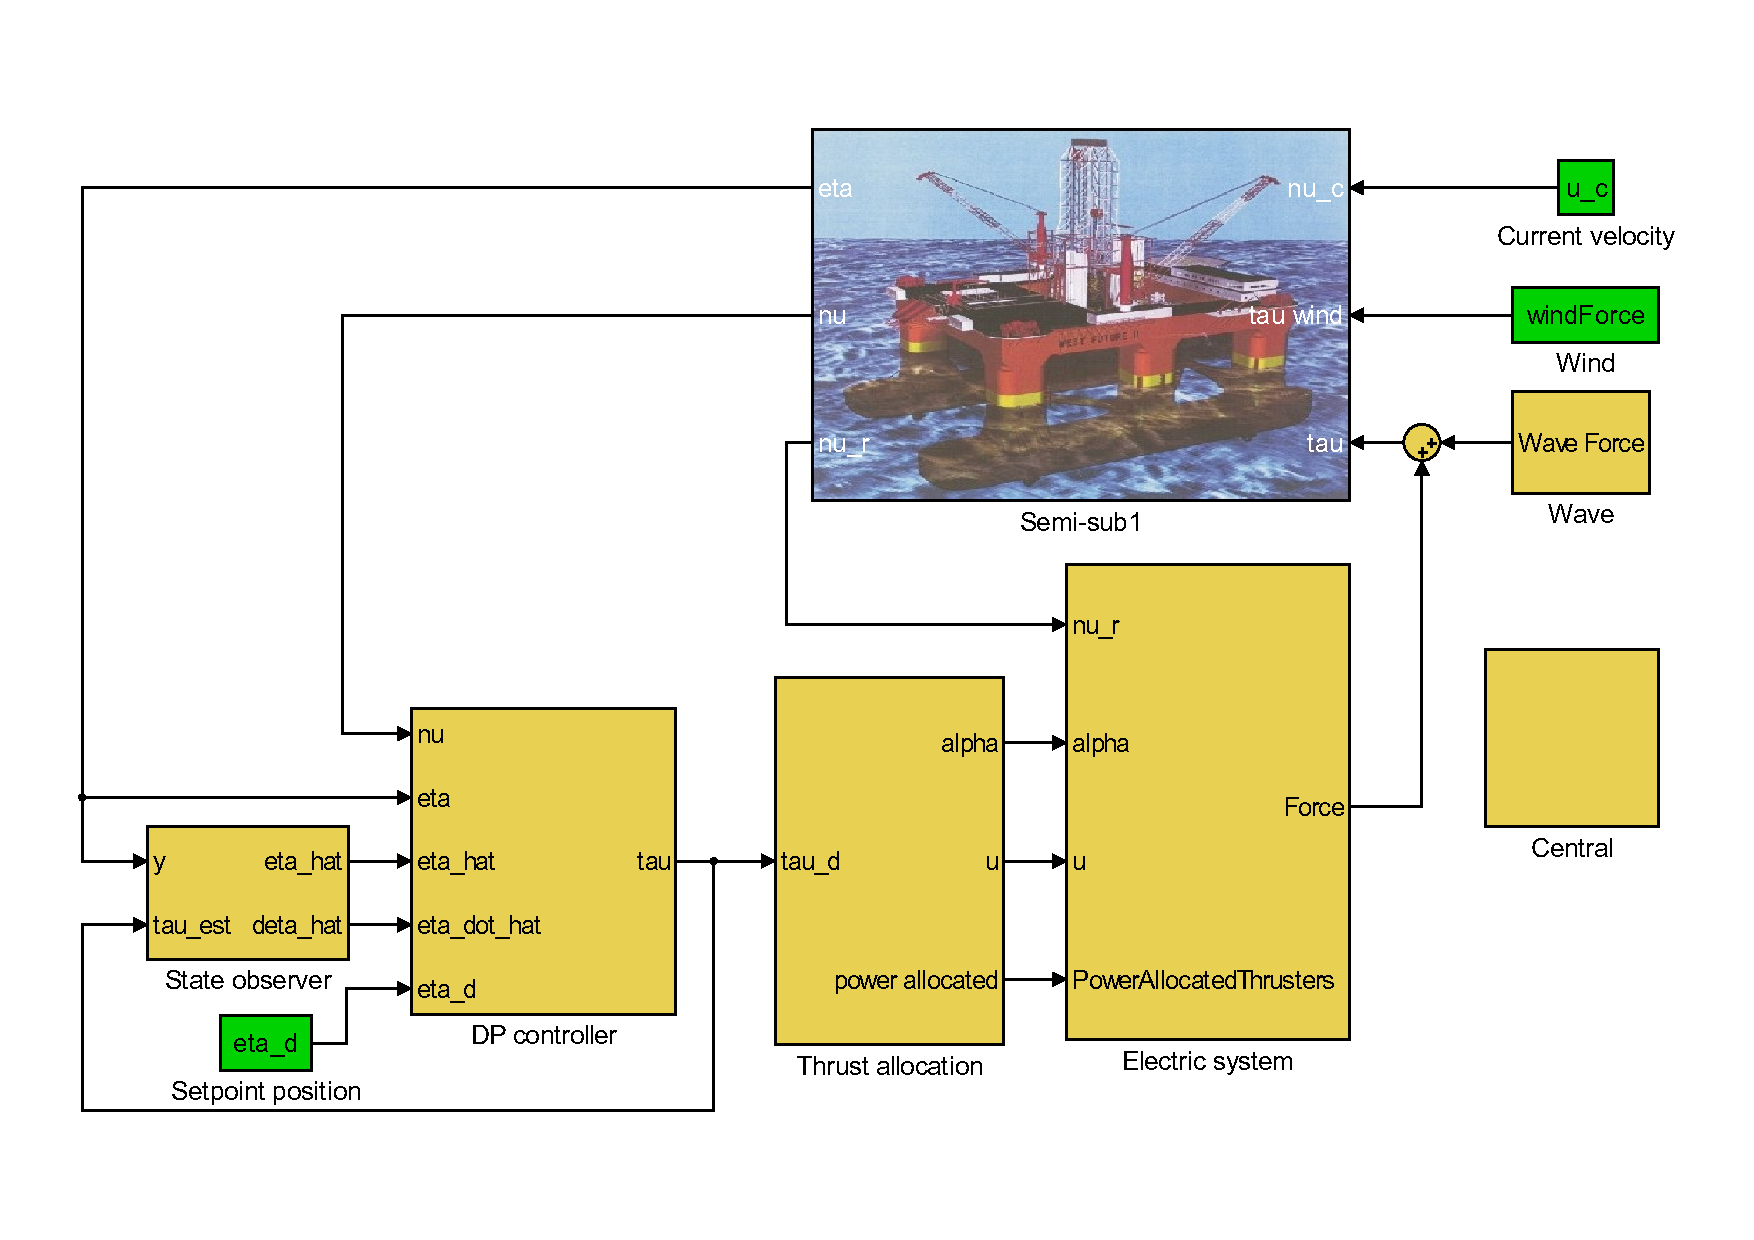
\includegraphics[trim=30 60 30 60,width=.7\textwidth,clip]{./figures/DPscheme}
\caption{Example of motion control view, top level view. 
The example shows the vessel model, observer, DP-controller, thrust allocation, and the electrical system.
The electrical system is further presented in Fig.~\ref{fig:PowerPlantsscheme}.}
\label{fig:DPscheme}
\end{figure*}

For this particular case the view contains:\begin{enumerate}
\item Observer; estimates the position and velocity of the vessel from measurements.
\item DP control system; calculates a desired thrust command.
\item Thrust allocation (TA); converts the desired thrust command for the vessel to thrust commands for each thruster.
\item Electric system with thruster model; converts the thrust command to actual thrust.
\item Environmental model; generates realistic current, wind, and wave loads for the environment.
\item Vessel model; calculates the motions of the vessel given the thruster and environmental loads.
\end{enumerate} 

The electric power plant is modeled inside the electric system block.
An example power plant is shown in Fig.~\ref{fig:PowerPlantsscheme} and consists of:
\begin{enumerate}
\item Generator set; consisting of a prime mover (e.g., diesel engine), a generator, a speed governor, and an automatic voltage regulator (AVR).
\item Thruster drives; consisting of a frequency converter, an electric motor, and a propeller.
\item Other components: This can be hotel loads and drilling loads, which are modeled as a time series of power consumption. However, this block may also be used for energy storage, such as batteries with a frequency converter. The load is then negative when the block delivers power and positive when it consumes power.
\item Switchboards; connecting loads and producers.
\item Breakers; connecting and disconnecting elements.
\end{enumerate}


\begin{figure*}[t!]
\centering
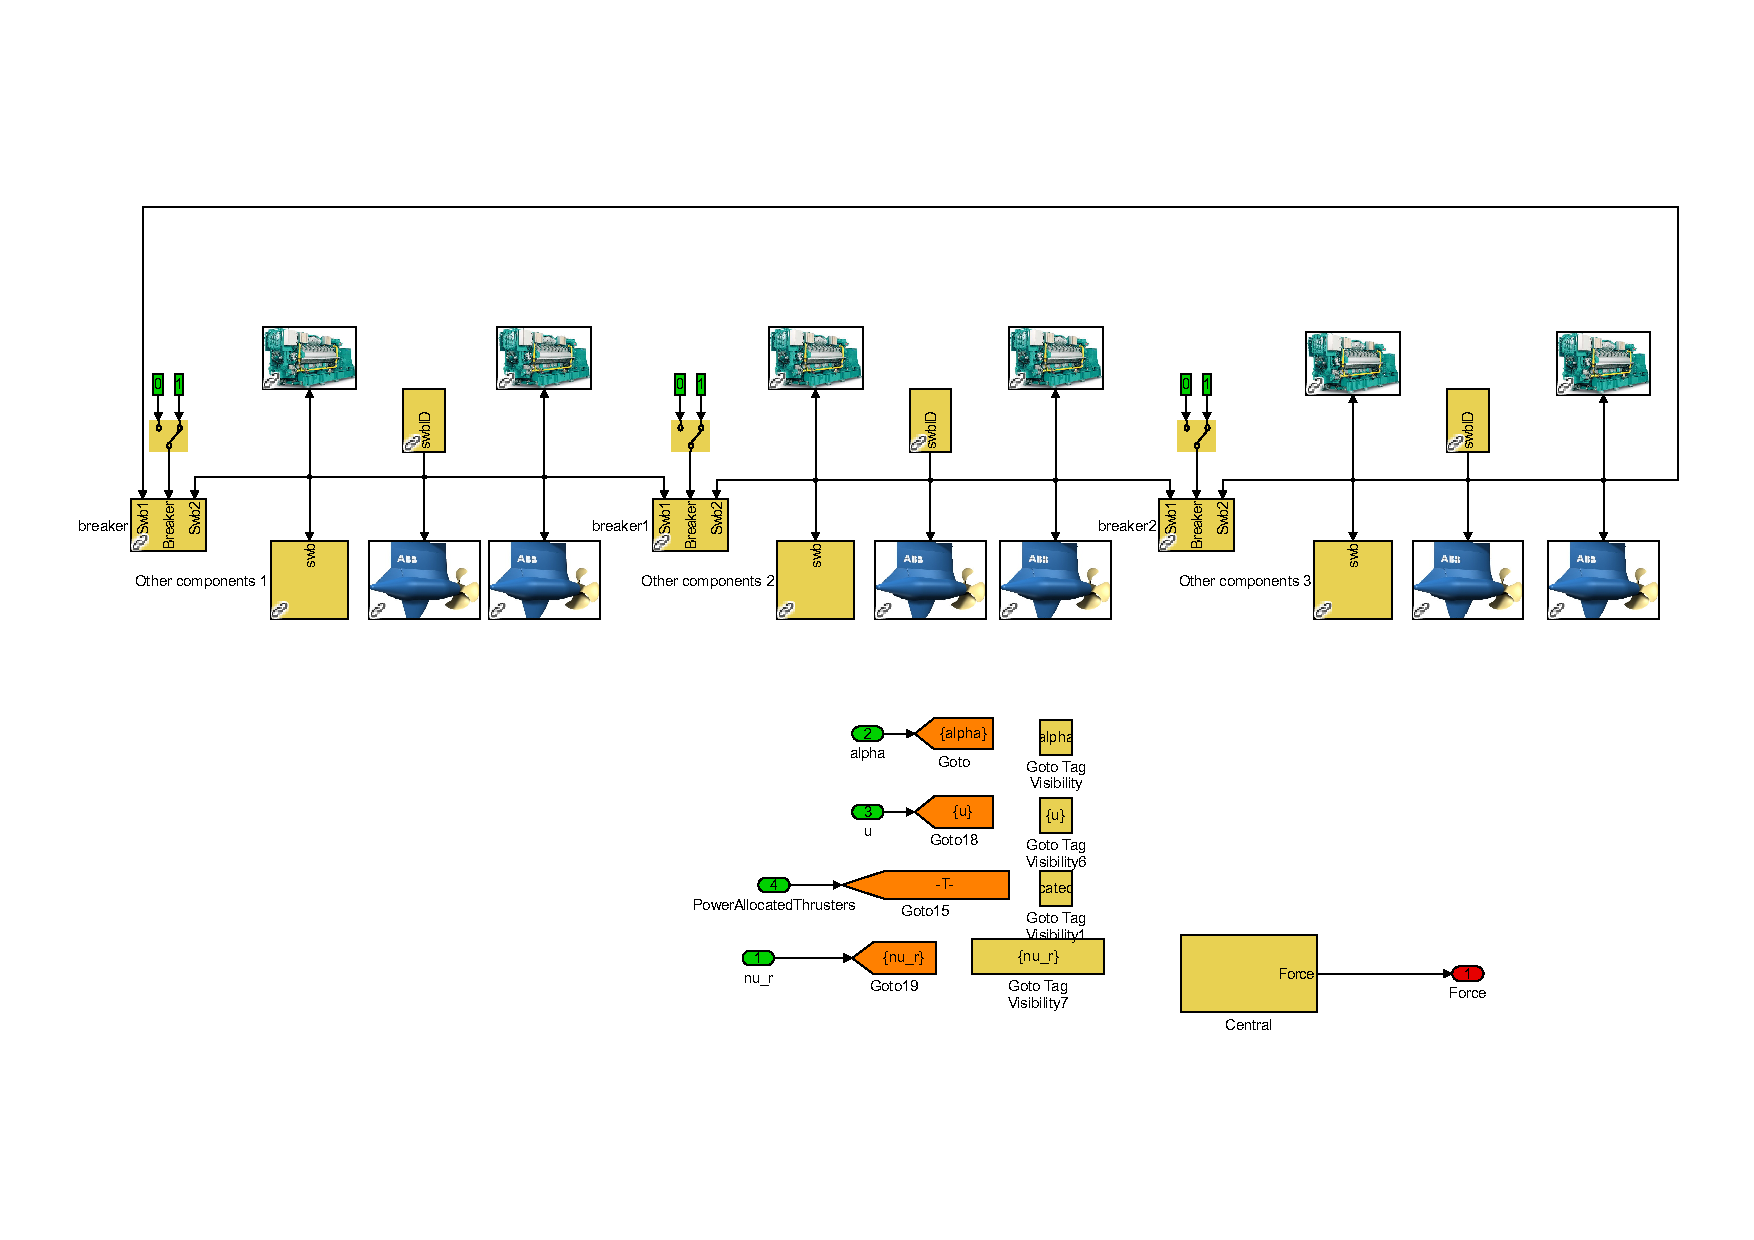
\includegraphics[trim=30 280 30 80,width=\textwidth,clip]{./figures/elscheme.pdf}
\caption{Example of power plant view. Includes the bus tie breakers, thrusters, generatorsets, and other loads block.}
\label{fig:PowerPlantsscheme}
\end{figure*}



Simulink was chosen because we would like to extend MSS~toolbox~\cite{MSS} to include better thruster models and an electric power plant.
The downside by choosing Simulink is the modeling of interconnections.
The system is hard to divide into levels as required by the subsystem architecture of Simulink.
We have therefore chosen to use the top level model view for the vessel control, further the electric power plant is a subsystem in this view.
The electric power plant is made to mimic a single line diagram.
However, no information other than the configuration is sent via the lines in Simulink.
Goto blocks are used to send information between the blocks to avoid a ``spagetti'' diagram with too many lines.
A script is used to automate the configurations of the goto blocks.
The stiff solver ode15s is used as numerical solver in the case study, since the local controllers gives a stiff model.
When the models are exported from Simulink to cRIO, the solver ode3 with step sizes of 1~millisecond is used, as cRIO does not support variable timestep solvers.

First order lowpass filters are used to avoid algebraic loops, where the time constant of the filters are chosen to be smaller than the fastest dynamics of the relevant models.
One example is the power available signal.
An algebraic loop occurs since the power available is dependent on the power consumption, which is constrained by the power available.
This is solved by adding a lowpass filter on the power available signal, which is faster than the time scale of the consumers.
This may also be solved by using discrete time for these signals.
However, this reduces the performance of the chosen implicit ode solver.

\section*{\uppercase{Vessel, Environment, Observer and DP-controller}}
The vessel model used in the simulator is from the MSS toolbox~\cite{MSS}.
In the simulation case we have chosen a model suitable for DP~operations.
However, the MSS toolbox contains multiple vessels models, and the model should be chosen depending on the simulation case.

The environment can be modeled as any external force.
The current is modeled as a relative velocity.
In the simulations presented in the case study below, the wave and wind loads are for simplicity modeled as sinusoidal forces with a constant bias.
This represents the mean wind force and waves (swells).
For cases where the DP~performance should be studied deeper, a higher fidelity model of the environment is needed.
This is given in the MSS toolbox.
The state observer is a passive observer based on~\cite{Fossen19993}, and the DP-controller is implemented as a PID-controller.

The thrust allocation (TA) calculates thrust demands for the thrusters, such that the sum equals the desired thrust command from DP.
Constraints are also applied, such as rate constraints and power constraints.
To maximize the fuel efficiency and increase flexibility, azimuth thrusters, i.e., thrusters that can change their direction of thrust, are often used.
The implemented TA is based on~\cite{Ruth2009,Johansen2013,Veksler2014a}.

%The total thrust must be equal to the desired thrust:
%\begin{equation}
%\vect{\tau}_d = T(\vect{\alpha}) \vect{f}
%\end{equation}
%where $\tau_d$ is the desired thrust commanded by the DP controller, $\vect{\alpha}$ is the azimuth angle of the thrusters, and $\vect{f}$ is the thrust command for each thruster which should be calculated by the TA.
%The thrust matrix $T(\vect{\alpha})$ gives the relationship between thrust of each thruster and the total thrust of the vessel (assuming no interaction and losses).

%We would like to make sure that the thrusters are able to produce force in any direction without rotating the thrusters, as it is faster to change the force of the thruster than rotating them.
%However, the optimal configuration of the thrusters is often a singularity point.
%This means that the thrusters are oriented such that they can not produce thrust in all possible directions without rotating at least one.
%For example, it is optimal to direct all thrusters to point forward if the thrust demand is in surge direction.
%Then the thrusters will not be able to produce thrust in sway direction.
%The determinant of $T(\vect{\alpha})$ is zero at the singularity point.
%The cost $\frac{\varrho}{\epsilon + |T(\vect{\alpha})|}$ is therefore added to avoid the singularity cost, where $\epsilon>0$ is a smoothing constant to avoid that the cost goes to infinity and $\varrho$ is cost weight.
%
%A nonlinear optimization problem is solved to minimize the power consumption of the thruster.
%The cost function is:
%\begin{equation}
%\begin{aligned}
%J(\vect{f},\vect{\alpha}) =& \vect{f}\tr H \vect{f} +  \left(\vect{f-f_0}\right)\tr G \left(\vect{f-f_0}\right) \\
% &+  \left(\vect{\alpha-\alpha_0}\right)\tr L \left(\vect{\alpha-\alpha_0}\right) +\frac{\varrho}{\epsilon + |T(\vect{\alpha})|}
%\end{aligned}
%\end{equation}
%where $H$ is a weight matrix, $\vect{f}$ are the magnitudes of the thrust of the thrusters, $\vect{\alpha}$ is the azimuth angle of the thrusters, $\vect{f_0}$ and $\vect{\alpha_0}$ are the previously applied force magnitude and azimuth angle, G and L are weight matrices for change of thrust magnitudes and azimuth angles.
%
%
%
%The power consumption of each thruster is approximated to:
%\begin{equation}
%p = K_{t2p} |f|^{1.5}
%\end{equation}
%A limit on how much power DP is allowed to use per bus is given by the PMS.
%This gives the constraint:
%\begin{equation}
%\sum\limits_{i=1}^{N_j}p_i \leq p^{(j)}_{max}
%\end{equation}
%where $N_j$ is the number of thrusters on bus~$j$, and $p^{(j)}_{max}$ is the power limit for bus~$j$.
%A power limit is also applied on each thruster:
%\begin{equation}
%K_{f2p} |f_i|^{1.5} \leq p_{max,i}.
%\end{equation}
%
%The thrusters have constraints on how fast they can change the azimuth angle and the thrust:
%\begin{align}
%|f-f_0| &\leq \Delta f_{max} \\
%|\alpha-\alpha_0| &\leq \Delta \alpha_{max}
%\end{align}
%where $\Delta f_{max}$ and $\Delta \alpha_{max}$ are the maximum change of thrust magnitude and azimuth angle between two update instants of the thrust allocation.
%
%The last equations give non-convex constraints if reverse thrust is allowed.
%This means that the overall problem is not convex.
%However, the optimization problem is convex if the thrust is constrained to be either positive or negative.
%The solution of the optimization problem is therefore found by checking all possible permutations of positive and negative direction and selecting the solution with the minimum cost.
%
%In addition, slack variables are implemented to make the problem feasible also when it is not possible to achieve the desired thrust.

The power consumption by the thruster is approximated by:
\begin{equation}
p = K_{f2p} |T_d|^{1.5}
\end{equation}
where $p$ is the approximated power consumption, $T_d$ is the thrust amplitude, and $K_{f2p}$ is a constant found from bollard pull tests.
Due to the approximation, the actual power consumption may be different from the approximated power consumption.
This means that the power consumption may be violated even though the solution satisfies the power constraint.
The thrusters are therefore given a power constraint based on the approximated power consumption in the thrust allocation.
This ensures that the thrusters do not use more power than available for the DP on each of the buses.

\section*{\uppercase{Power Management System}}
The PMS objective is to make sure there is always enough power available, to prevent a fault (blackout), and if it occurs to restore power as fast as possible.
The PMS starts additional generators when the excessive power capacity of the connected producers is too small.
In addition, the PMS allocates power to the different consumers.
This is done by first summing the current power capacity of the producers.
This is then shared among the consumers based on their desired power consumption and priority.
A signal, called ``Power Available'', is sent to some consumers, stating the maximum power limit for by the specific load.
Load shedding (disconnection of consumers) is done in extreme cases, when power reduction must be done quickly (e.g., close to underfrequency).

Fast load reduction is used in cases where the power consumption must be reduced, such as after an unexpected failure of a generator.
It reduces the load of the thruster drives, since they can change the power consumption quickly due to the frequency converters.

The PMS will also adjust the droop and isochronos load sharing parameters to adjust the load sharing.
This is done during progressive loading after connection of generator sets.
Progressive loading is implemented to ensure that the power generation of the new producer is slowly increased from no load to desired load sharing.

The PMS algorithm is implemented in~C++ and can easily be configured to different power plants.
The object oriented focus of the simulator is kept in the PMS implementation, so that new functionalities, such as automatic start and stop, easily can be added.

\section*{\uppercase{Diesel Engine}}
The dynamics of the diesel engine are the slowest dynamics of a diesel-electric power plant. 
Most modern diesel engines are turbocharged to provide increased power density. 
When a turbocharged diesel engine needs to increase its delivered power, more air is required into the cylinders to avoid incomplete combustion or visible smoke in the exhaust.
However, the response of the air system is rather slow, due to the rotating inertia of the turbocharger and the large air- and exhaust receivers, which gives rise to the \textit{turbo-lag}. 
In addition, increasing the fuel injection rises the temperature in the cylinder. 
The rate of change of fuel injection should be limited to avoid large thermal stresses.

Constraints are, therefore, added to the engine control output by the engine manufacturer to ensure that the fuel injection is not changed too fast, so that the engine is not damaged by a rapid change of temperature, and that the pressure in the inlet manifold is large enough to allow for a complete combustion. 
These constraints are in some cases conservative and the air dynamics may be neglected since the engine will always run with complete combustion due to these constraints.

\subsection*{Mean Value Model}
The main purpose of the diesel engine simulation model is to capture the air dynamics including pressure before the engine cylinder which can be related to the charge air available for combustion. 
In the mean value engine model, most of the physics in the engine system components are captured except for the in-cylinder process, i.e., the thermodynamic cycle of an internal combustion engine. The main components included in the model are an engine cylinder block, a turbocharger, a charge air cooler, an air receiver and an exhaust receiver. 
The implemented mean value engine model is based on the models presented in~\cite{Guzzella2010,Chow1999,Heywood1988,Zacharias1967,Yum2013,Pedersen2000}.

%The engine system including a turbocharging system is inherently a thermodynamic process with gas mixture as medium. Therefore, main variables of the system are pressure ($p$), temperature ($T$), fuel-air equivalent ratio ($F$) which are thermodynamic states. Also flow variables such as mass flow ($\dot{m}$) of gas, enthalpy flow or rate of change in internal energy ($\dot{E}$) and mass flow of burned-fuel within ($\dot{m}_b$) are necessary in order to describe the dynamics of the system. 
%
%A filling and empty method \cite{Chow1999} is used to construct the thermodynamic process model of the system. In this approach, the target model is constructed by placing control volumes in a series as configured in the real system and putting a flow restriction between adjacent control volumes. It is assumed that the thermodynamic state such as pressure and temperature are uniform within in a control volume and that there is no accumulation of mass in the flow restriction. Then, all the components fall into two categories: a thermodynamic control volume and a flow restriction. Generally, pipes, receivers and cylinders are in the first category where as any valve, compressor, turbine and heat exchangers are considered as flow restrictions. 
%
%Thermal control volumes determine the thermodynamic states of the system. They consist of two parts. The first one is a flow junction where mass conservation and the first law thermodynamics are implemented. The second part is the flow accumulation where the net rate of change in mass and energy are integrated. The integrated values are the mass ($m_{\text{CV}}$), the internal energy ($U_{\text{CV}}$) and mass of burned fuel ($m_{\text{f}}$) within the control volume, which are states of the system. Pressure and temperature are derived from a table of thermodynamic properties, such as the JANAF table\cite{Chase1998}, and by using the equation of state (i.e. ideal gas law). In order to achieve faster simulation speed, a semi-empirical formula for thermodynamic properties found in \cite{Zacharias1967} is used in place of the table. 
%
%A flow restriction, placed in between two control volumes, determines the flow rate of mass and energy between them. The flow rate depends on pressure and temperature of the adjacent control volumes. In many cases, the equations of the equivalent ideal flow for compressible gas is used for this purpose. The equation used for the model is given in \cite{Heywood1988}. The equation, however, assumes isentropic process across the restriction. Therefore, any forms of energy gain or loss should be accounted in order to achieve the conservation laws. 
%
%In case of a compressor and a turbine, the model requires a performance data map from measurement or a manufacturer. The map represents the relationship between the pressure ratio across the device ($\Pi$) and rotating speed of the rotor ($\omega_\text{TC}$) versus the corrected mass flow ($\dot{m}_{\text{corr,TC}}$) and the isentropic efficiency of the process ($\eta_{\text{TC}}$). Having acquired the mass flow and the efficiency, the energy flow in and out can be calculated assuming the isentropic process. Then the torque for each turbomachine can be calculated as:
%\begin{equation}
%  Tq = \frac{\dot{m} \Delta h}{\omega_{TC}}
%\end{equation}
%A dynamic equation is used for the mechanical rotation of the turbocharger.
%\begin{equation}
%J\dot{\omega} = Tq_{turb} - Tq_{comp}
%\end{equation}
%
%The whole engine block including intake and exhaust valves, fuel injection system, cylinders and pistons is simplified to a single flow restriction model. In this model, the input is the pressure and temperature of the air receiver ($p_{AR},T_{AR}$), the engine speed ($\omega_\text{eng}$) and the fuel rack position ($u$). Mass flow through this restriction model can be determined with a volumetric efficiency ($\eta_\text{vol}$) of the process known. 
%\begin{equation}
%\begin{aligned}
%{{\dot m}_{in}} &= {\eta _\text{vol}}\left( {{p_\text{AR}}} \right) \cdot {\rho _\text{AR}}{V_d}\frac{{{\omega _{{\text{eng}}}}}}{{ns \cdot \pi }} \\
%{{\dot m}_{out}} &= {{\dot m}_{in}} + {{\dot m}_{b}} \\
%{{\dot m}_{b}} &= u \cdot {m_{f,\max }}\frac{{{\omega _{{\text{eng}}}}}}{{ns \cdot \pi }} 
%\end{aligned}
%\end{equation}
%where $\rho_\text{AR}$ is density of the gas in the air receiver, $ns$ is the number of stroke of the engine cycle and ${m_{f,\max }}$ is maximum amount of fuel injected per cycle.
%Energy flow in and out of the cylinder is also calculated as following.
%\begin{equation}
%\begin{aligned}
%{{\dot E}_{in}} &= {{\dot m}_{in}}{h_\text{AR}}\left( {{p_\text{AR}},{T_\text{AR}}} \right) \\
%{{\dot E}_{out}} &=  \dot E_{in}+ {{\dot m}_{b,out}}LHV\left( {1 - {C_{HT}} - \frac{{3.6{\text{e}}9}}{{LHV \cdot SFC}}} \right)
%\end{aligned}
%\end{equation}
%where $LHV$ is low heating value of the fuel and $C_{HT}$ is the heat transfer ratio and $SFC$ is the specific fuel consumption in unit of g/kWh. 
%The torque output of the engine, then, can be determined. 
%\begin{equation}
%{T_q} = \frac{{3.6{\text{e}}9 \cdot {{\dot m}_{b,out}}}}{{SFC \cdot {\omega _{{\text{eng}}}}}}
%\end{equation}
%
The overall mean value engine system model is presented in Figure \ref{fig:MVEMscheme}.
Both a compressor model and a turbine model require ambient pressure and temperature as boundary conditions for the system. The input to the overall model is fuel rack position and engine speed; the output is torque, volumetric efficiency and pressure and temperature of the air receiver. 
The latter three outputs are used in order to calculate the mass trapped in the cylinder per cycle, which is further used to calculate the maximum allowable injected fuel amount according to given fuel-air equivalent limit. This functionality is termed as smoke limiter. 
The smoke limiter ensures that the charge in the cylinder is lean enough to avoid visible smoke during rapid power output increase. 
\begin{figure}
\normalsize
\centering
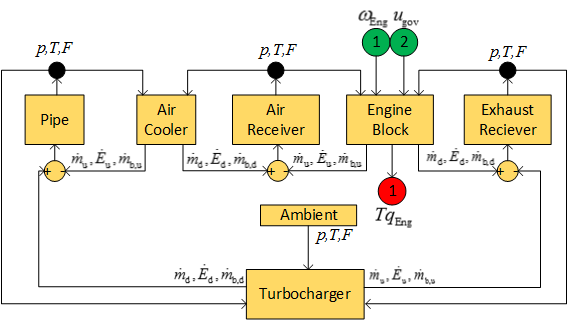
\includegraphics[width=0.45\textwidth]{./figures/MVEMScheme.png}
\caption{Mean value engine system model scheme, including a turbocharger, a charge air cooler and incylinder process.}
\label{fig:MVEMscheme}
\end{figure}

A short-coming of such a model is that it requires extensive parameter identification in order to achieve reasonable accuracy. However, a well-defined engine model can be used for different cases if the main physical variables are converted into per unit values. This may cause inaccurate response characteristics since machines at a various power range should have somewhat different time scales. If it is possible to find the response characteristics of a genset to step load changes, the overall model including the governor can be re-tuned to match the given characteristics. Such characteristics can be found in the manufacturer's documentation\cite{MANEnginesandSystems2013}.

\subsection*{Rate Constrained Model}
A simplified model can be used for engines where the fuel rate is constrained such that the combustion is complete.
Simulations (not shown due to page limitations) have shown that this is the case for maritime engines, due to the conservative rate constraints set by the engine manufactures.
This model ignores the air dynamics and requires therefore fewer parameters.

The shaft speed dynamics can therefore be simplified to:
\begin{align}
\dot{\theta} =& \omega \omega_b\\
\dot{\omega} =& \frac{1}{2H} \left(-D_f \omega + k_u u - \tau_e \right)
\end{align}
where $\theta$ is the mechanical angle, $\omega$ and $\omega_b$ is the per unit and base mechanical angular velocity, $D_f$ denotes windage friction constant, $k_u$ is a gain from fuel rate to per unit mechanical torque, $\tau_e$ denotes per unit electric torque, and $u$ is the fuel index.
This is derived by the swing equation and assuming linear damping.
H is the inertia constant, defined as
$
H = \dfrac{1}{2}\dfrac{J \omega_b^2}{P_b}
$,
where $J$ is the rotational inertia of the generator set and $P_b$ is the base power of the generator set~\cite{Krause2002}.

\subsection*{Governor}
The two engine models use the same governor, which is based on droop control~\cite{Woodward2004}.
The commanded fuel index is then calculated by a PID controller with back calculation to avoid wind-up of the integrator term.
The derivative of the frequency is calculated by using the ``dirty derivative'':
\begin{align}
&\omega_{ref} = \omega_{NL}-K_{droop}p \\
&u = K_p (\omega_{ref}-\omega)+K_i \xi - K_d \hat{\dot{\omega}}\\
&\dot{\xi} = \omega_{ref}-\omega + K_b(u_{saturated}-u)\\
&\hat{\dot{\omega}}= N(\omega-\hat{\dot{\omega}}) 
\end{align}
where $K_d$, $K_i$, and $K_p$ are the derivative, integration, and proportional gains; $p$ is the per unit produced power by generator; $\omega_{NL}$ and $\omega_{ref}$ are the set-point frequency at zero active power and reference frequency; and $\hat{\dot{\omega}}$ denotes the estimated time derivative of the frequency.

For the rate constraint model, additional constraint on the fuel index is needed to avoid too large temperature variations in the cylinder and sooting due to too little air for complete combustion. This constraint is pre-defined and, therefore, static. In the case study, the engine is allowed to increase the fuel index with 20~\% of the rated output and then increase the fuel index with $8.1 \%/s$. This is found by tuning the engine model response to best fit recovery time and frequency droop given in \cite{MANEnginesandSystems2013}.

For the mean value model, a smoke limiter put constraint over the governor's command. Given the maximum fuel-air equivalent ratio ($F_\mathrm{max}$), the maximum fuel index ($u_{max}$) is given by the equation \ref{eq:maxFIndex},

\begin{equation}
\label{eq:maxFIndex}
u_\mathrm{max} = \eta_\mathrm{vol}\frac{p_\mathrm{rec}V_{D}}{RT_\mathrm{rec}} \frac{F_\mathrm{max}f_s}{m_\mathrm{f,inj}}
\end{equation}
where, $\eta_\mathrm{vol}$ is volumetric efficiency, $p_\mathrm{rec}$ and $T_\mathrm{rec}$ are pressure and temperature at an air reciever, $R$ is specific gas constant and $V_D$ is displacement volume of a a cylinder, $f_s$ is stoichiometric fuel-air ratio and $m_\mathrm{f,inj}$ is amount of maximum fuel injection per cycle. In the case study, the $F_\mathrm{max}$ is chosen as 1 in order to give a reasonable engine response.

\section*{\uppercase{Generator}}
In marine power plants, synchronous generators are typically used to produce power.
As earlier mentioned, the generator is assumed to be in steady state and with balanced phases.
The electrical torque, $\tau_e$ is therefore 
\begin{equation}
\tau_{e} = \dfrac{p+p_{loss}}{\omega} = \dfrac{p}{\omega}+\dfrac{r(p^2+q^2)}{\omega v^2}
\end{equation}
where $p_{loss}$ is the power loss in the generator, $r$ is the resistance in the stator windings, $q$ is the reactive power, and $v$ is the terminal voltage.
From \cite{Krause2002}, we know that the terminal line-to-neutral voltage is:
\begin{equation}
\tilde{V}_a=-Z \tilde{I}_a+\tilde{E}_a
\end{equation}
where $Z$ is the internal impedance of the generator set, $\tilde{I}_a$ is the current through phase $a$ and $\tilde{E}_a$ is the induced line-to-neutral voltage for phase $a$.

It is assumed that the magnitude of $\tilde{E}_a$ is perfectly controlled by the automatic voltage regulator (AVR) or at least the dynamics are much faster than the dynamics of the mechanical system.
The phase angle of $\tilde{E}_a$ is
\begin{equation}
\angle{\tilde{E}_a} = \frac{\theta N_{poles}}{2}
\end{equation}
where $N_{poles}$ is the number of poles of the generator.

The AVR regulates the terminal voltage by manipulating the induced voltage.
In this simulator we use a droop controller to set the set-point, based on the reactive power of the generator set.
This takes care of the reactive load sharing. 
The generators deliver equal amount of reactive power if they have equal voltage droop curves.

\section*{\uppercase{Electric Voltage Calculation}}
\label{sec:voltage}
The voltage of the bus is needed to calculate the load sharing of the generators.
The generators are connected in parallel as shown in Fig.~\ref{fig:circuitbus}.
We assume that the loads are independent of the bus voltage, their active and reactive power are therefore given.
To calculate the bus voltage we first find a Th\'{e}venin equivalent circuit of the connected generator sets~\cite{rizzoni2007}, as shown in Fig.~\ref{fig:circuitThevenin}.
This circuit is closed by the loads, which have a known power consumption but unknown impedance.

\begin{figure}
\begin{circuitikz}[american voltages]
\draw
(0,0) to [short] (6.5,0)
to [sV, l_=$\tilde{E}_{a,n}$] ++(0,1.5)
to [R, l_=$Z_n$] ++(0,1.5)
(6.5,4) to [short, i_=$\tilde{I}_{a,n}$] ++(0,-1)
(6.5,4) to [short] (0,4)
(0,0) to [vR, l_=$Z_{load}$] (0,4)

(4,0)  to [sV, l_=$\tilde{E}_{a,2}$] ++(0,1.5)
to [R, l_=$Z_2$] ++(0,1.5)
++(0,1) to [short, i_=$\tilde{I}_{a,2}$] ++(0,-1)

(2,0)  to [sV, l_=$\tilde{E}_{a,1}$] ++(0,1.5)
to [R, l_=$Z_1$] ++(0,1.5)
++(0,1) to [short, i_=$\tilde{I}_{a,1}$] ++(0,-1)
node (A) at (-.25,0) {}
node (B) at (-.25,3.5) {}
(A) to [open, v^>=$\tilde{V}$] (B);
\node at (5.25,2) {...};
\end{circuitikz}
\caption{Circuit diagram of bus with one load with the impedance $Z_{load}$ and $n$ gerators.}
\label{fig:circuitbus}
\end{figure}

\begin{figure}
\centering
\begin{circuitikz}[american voltages]
\draw
(0,0) to [short] (3,0)
to [sV, l_=$\tilde{E}_{T}$] ++(0,1.5)
to [R, l_=$Z_T$] ++(0,1.5)
(0,4) to [short] (3,4)
to [short, i_=$\tilde{I}$] ++(0,-1)
(0,0) to [vR, l_=$Z_{load}$] (0,4)
node (A) at (-.25,0) {}
node (B) at (-.25,4) {}
(A) to [open, v^>=$\tilde{V}$] (B);
\end{circuitikz}
\caption{Thevenin equivalent circuit of generators connected to bus as shown in Fig.~\ref{fig:circuitbus}.}
\label{fig:circuitThevenin}
\end{figure}
This gives the equation 
\begin{equation}
P_{bus}+j Q_{bus} = 3 \tilde{V} \tilde{I}^* = 3 \tilde{V} \frac{\tilde{E}^*_T-\tilde{V}^*}{Z_T^*}
\label{eq:powerBus}
\end{equation}
where $P_{bus}$ and $Q_{bus}$ is the active and reactive power of the loads, $\tilde{V}$ is the line-to-neutral bus voltage, $\tilde{I}$ is the current, $\tilde{E}_T$ is the Th\'{e}venin equivalent voltage, and $Z_T$ is the Th\'{e}venin equivalent impedance.
Equation~\eqref{eq:powerBus} has two solutions, one solution, or no solution.
For the case where there exists two solutions the solution with the largest absolute value for the bus voltage is used.
The largest voltage yields a low current, hence low internal loss.
The lower voltage solution gives a high current, with very high internal loss since most of the voltage drop occurs over the internal impedance.

During simulations it may occur that there doesn't exist a valid solution. This may happen when the load increases rapidly (a load is connected) or the Th\'{e}venin equivalent voltage of the generator decreases rapidly (fault in AVR or disconnection of a generator).
In such cases, the voltage is set to a low value.
This gives an incorrect load sharing, but the AVR will increase the voltage quickly.
During our simulation study the bus voltage has regained a valid solution within 0.1 millisecond (not shown in article due to page limitations).
This is permissible since the time is very short compared to the time scale of the mechanical system.
A lowpass filter must therefore be added when simulating voltage protection relays.

\section*{\uppercase{Thrusters}}
The thrusters are modeled as propellers which is driven by electrical motors.
The propellers are assumed to be fixed pitch, while the speed is variable.
No thruster-thruster or thruster-hull interaction losses are included, as these are generally hard to describe.
It is assumed that the torque of the electrical motor is perfectly controlled.
A frequency controller is often used to control the motor.
The time scale of the dynamics of the frequency converter is much faster than the dynamics of the mechanical part of the thruster drives, and can therefore be neglected.
A speed controller is used to control the thrust. 
The open water characteristics are used to calculate the desired shaft speed, from the requested thrust.
The thrust is assumed to be~\cite{Sorensen2011}:
\begin{equation}
T_a = \operatorname{sign}(n)K_T \rho D^4 n^2 
\end{equation}
where $K_T$ is the thrust coefficient found from open water tests, $\rho$ is the density of water, $D$ is the propeller diameter, and $n$ is the shaft speed.
This gives the desired shaft speed:
\begin{equation}
n_d = \operatorname{sign}(T_d) \sqrt{\frac{|T_d|}{K_T \rho D^4}}
\end{equation}

The desired thrust signal must be smoothed since the desired thrust is calculated at 1~Hz.
Large power fluctuation will occur at each update instant of the thrust allocator if this is not done.
A second order filter is therefore used, to make the desired thrust signal smooth.

The power consumption of the thrusters are reduced after a fault by the fast load reduction.
This is done by limiting the torque of the electrical motor driving the propeller.
In practice, this is done by the frequency converter.

The four-quadrant model of the propeller presented in~\cite{Smogeli2006}, is used to calculate the actual thrust and torque of the thruster.
The benefit of this model is that it models ``wind milling'' (i.e., shaft speed and torque have different signs).
The advance velocity of the propeller is assumed to be equal to the relative velocity of the vessel.
This means that wave-propeller interaction due to vessel motion is included, but wave-propeller interaction due to wave induced particle motion is not included~\cite{Sorensen2009}.

%This model was first presented by~\cite{Miniovich1960}. 
%The thrust and torque coefficients are defined as:
%\begin{align}
%C_T =& \frac{T_a}{\frac{1}{2}\pi R^2 \rho V_{0.7}^2} \\
%C_Q =& \frac{Q_a}{\frac{1}{2}\pi R^3 \rho V_{0.7}^2}
%\end{align}
%where $T_a$ is the thrust, $R$ the radius of the propeller, and $Q_a$ is the propeller torque. $V_{0.7}$ is the undisturbed incident velocity to the propeller blade at radius $0.7R$ and is defined as:
%\begin{equation}
%V_{0.7}=\sqrt{V_a+(0.7\omega R)^2}
%\end{equation}
%where $\omega$ is the angular velocity of the propeller shaft.
%
%The angle of attack of the propeller at $0.7R$, $\beta$, is defined as:
%\begin{equation}
%\beta = \arctan\left(\frac{V_a}{0.7 \omega R}\right)
%\end{equation}
%To estimate $C_T$ and $C_Q$ a Fourier approximation as a function of $\beta$ is used, with parameters from~\cite{Smogeli2006}.


\section*{\uppercase{Other Components}}
The last model in the electrical power simulator is a block named \textit{other loads}.
It represents loads that does not directly influence the propulsion system and are modeled as time series of actual and desired power consumption.
The load is divided into two parts: high and low priority loads.
Both send a desired power consumption to the PMS.
The PMS will then allocate power available back to these loads.
The PMS will first allocate power to the high priority loads, which may be an emergency system.
The thrusters will then get allocated the remaining power, before the low priority loads get the last remaining available power.
The actual consumed power is set equal to the allocated power available.



\section*{\uppercase{Real-time Implementation}}
One National Instruments compact reconfigurable input/output (cRIO) embedded control and acquisition systems is used for the real-time implementation.
This gives the opportunity to run hardware-in-the-loop testing where simulated models are replaced by real hardware.
This could be controllers or other components, such as generator sets.

\section*{\uppercase{Case Study}}
In this article a drilling rig is used to illustrate the capabilities of the simulator for a fault scenario.
The electrical system is shown in Fig.~\ref{fig:PowerPlantsscheme}.
The rig has three switchboards, which are connected in a ring configuration.
Two generator sets are connected to each switchboard, where the rated output of the diesel engines are 9.1~MW.
In addition, two thrusters are connected to each switchboard with a rated output of 4.2~MW and a rated thrust of 506~kN.
The current velocity is set to 1~m/s and the wind force is constant at 437~kN, both are coming from north.
In the simulation, the vessel is in DP~operation and heading north, with closed bustie and five generator sets running (two connected to each of the first two switchboard and one to the righter most switchboard).
Switchboard~1 is separated from the other two switchboards, by opening the breakers connected to Switchboard~1 after 50~seconds.
The power consumption is constrained by the fast load reduction, due to the increased load on Switchboard~2 and~3.
50~seconds later, the last generator connected to Switchboard~3 is disconnected.
A thruster connected to Switchboard~3 is disconnected 2 seconds after the disconnection of the generator.
To avoid underfrequency the fast load reduction reduces the thrust.
The PMS uses the power available signal to avoid overload of the generators after the fast load reduction has increased its constraints.
The thrust allocation is then able to redistribute the thrust between the buses, since the power available signal is directed to the thrust allocation.

As is seen in Fig.~\ref{fig:caseplot} we are able to simulate this fault scenario.
We are also able to simulate how the safety systems respond and how this influence the position accuracy and power plant.
Also note that the power consumption of the thrusters are fluctuating before the faults occur.
This is due to the wave induced motions of the vessel, which gives fluctuating advance velocity of the propeller.
Switchboard~1 is also increasing its thruster loads after the loss of a generator and thruster at Switchboard~3.
This is done since the thruster loads is at the power available limit for Switchboard~2 and~3.
Some position deviation from the setpoint occurs after the fault; this is due to the reconfiguration and loss of power after the fault.

\begin{figure}
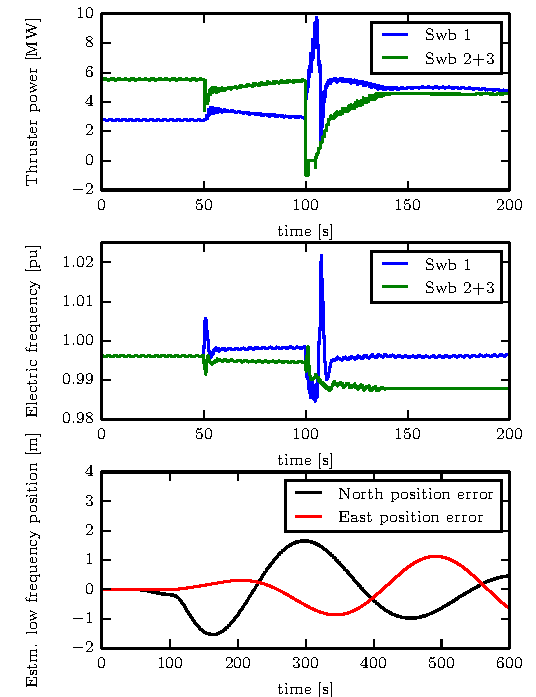
\includegraphics{figures/omae}
\caption{Power consumption of thrusters, electric frequency, and position deviation from DP~set-point for simulation presented in section ``Case study''}
\label{fig:caseplot}
\end{figure}


%\section*{\uppercase{Further Work}}
%Such a simulator as presented can always be extended to higher fidelity and include new models and control strategies.
%Some models which may be added are low level protection system, such as undervoltage/-frequency relay.
%The simulator is not able to connect two buses during a simulation since the switchboards may not be synchronized.
%To be able to do so a bus synchronizer is needed, which will adjust the no load frequency of the generator sets.


\section*{\uppercase{Conclusion}}
\label{sec:conclusion}
In this article a simulator for marine vessels' electric propulsion is presented.
The main contributions are a system simulator with detailed models of the vessel, propeller, thruster drives, generator sets, and controllers, in addition to including interaction effects between the components.
The simulator is module based and models of different fidelity can be chosen.
Due to the modularity the simulator can be reconfigured to many different vessels with electric propulsion, and different operations can be simulated.
Simulink is used to implement the simulator and the simulator can run on NI cRIO in real-time.
The case study presented in the article shows some of the capabilities of the simulator. More detailed simulations of, e.g.,  fault scenarios contribute to increased knowledge about the behavior of the electrical system and safety functions, which may lead to more reliable vessels and safer operations in the future. 



%%%%%%%%%%%%%%%%%%%%%%%%%%%%%%%%%%%%%%%%%%%%%%%%%%%%%%%%%%%%%%%%%%%%%%
\begin{acknowledgment}
The authors of this paper are funded by the project Design to verification of control systems for safe and energy efficient vessels with hybrid power plants (D2V), where the Research Council of Norway is the main sponsor. NFR: 210670/070, 223254/F50
This work was also partly supported by the Research Council of Norway through the Centres of Excellence funding scheme, project number 223254 - AMOS
\end{acknowledgment}




%%%%%%%%%%%%%%%%%%%%%%%%%%%%%%%%%%%%%%%%%%%%%%%%%%%%%%%%%%%%%%%%%%%%%%
% The bibliography is stored in an external database file
% in the BibTeX format (file_name.bib).  The bibliography is
% created by the following command and it will appear in this
% position in the document. You may, of course, create your
% own bibliography by using thebibliography environment as in
%
% \begin{thebibliography}{12}
% ...
% \bibitem{itemreference} D. E. Knudsen.
% {\em 1966 World Bnus Almanac.}
% {Permafrost Press, Novosibirsk.}
% ...
% \end{thebibliography}

% Here's where you specify the bibliography database file.
% The full file name of the bibliography database for this
% article is asme2e.bib. The name for your database is up
% to you.
\bibliographystyle{asmems4}
\bibliography{main}

%%%%%%%%%%%%%%%%%%%%%%%%%%%%%%%%%%%%%%%%%%%%%%%%%%%%%%%%%%%%%%%%%%%%%%
\appendix       %%% starting appendix
\end{document}
